% Options for packages loaded elsewhere
\PassOptionsToPackage{unicode}{hyperref}
\PassOptionsToPackage{hyphens}{url}
\PassOptionsToPackage{dvipsnames,svgnames,x11names}{xcolor}
%
\documentclass[
  letterpaper,
  DIV=11,
  numbers=noendperiod]{scrartcl}

\usepackage{amsmath,amssymb}
\usepackage{iftex}
\ifPDFTeX
  \usepackage[T1]{fontenc}
  \usepackage[utf8]{inputenc}
  \usepackage{textcomp} % provide euro and other symbols
\else % if luatex or xetex
  \usepackage{unicode-math}
  \defaultfontfeatures{Scale=MatchLowercase}
  \defaultfontfeatures[\rmfamily]{Ligatures=TeX,Scale=1}
\fi
\usepackage{lmodern}
\ifPDFTeX\else  
    % xetex/luatex font selection
\fi
% Use upquote if available, for straight quotes in verbatim environments
\IfFileExists{upquote.sty}{\usepackage{upquote}}{}
\IfFileExists{microtype.sty}{% use microtype if available
  \usepackage[]{microtype}
  \UseMicrotypeSet[protrusion]{basicmath} % disable protrusion for tt fonts
}{}
\makeatletter
\@ifundefined{KOMAClassName}{% if non-KOMA class
  \IfFileExists{parskip.sty}{%
    \usepackage{parskip}
  }{% else
    \setlength{\parindent}{0pt}
    \setlength{\parskip}{6pt plus 2pt minus 1pt}}
}{% if KOMA class
  \KOMAoptions{parskip=half}}
\makeatother
\usepackage{xcolor}
\setlength{\emergencystretch}{3em} % prevent overfull lines
\setcounter{secnumdepth}{5}
% Make \paragraph and \subparagraph free-standing
\makeatletter
\ifx\paragraph\undefined\else
  \let\oldparagraph\paragraph
  \renewcommand{\paragraph}{
    \@ifstar
      \xxxParagraphStar
      \xxxParagraphNoStar
  }
  \newcommand{\xxxParagraphStar}[1]{\oldparagraph*{#1}\mbox{}}
  \newcommand{\xxxParagraphNoStar}[1]{\oldparagraph{#1}\mbox{}}
\fi
\ifx\subparagraph\undefined\else
  \let\oldsubparagraph\subparagraph
  \renewcommand{\subparagraph}{
    \@ifstar
      \xxxSubParagraphStar
      \xxxSubParagraphNoStar
  }
  \newcommand{\xxxSubParagraphStar}[1]{\oldsubparagraph*{#1}\mbox{}}
  \newcommand{\xxxSubParagraphNoStar}[1]{\oldsubparagraph{#1}\mbox{}}
\fi
\makeatother


\providecommand{\tightlist}{%
  \setlength{\itemsep}{0pt}\setlength{\parskip}{0pt}}\usepackage{longtable,booktabs,array}
\usepackage{calc} % for calculating minipage widths
% Correct order of tables after \paragraph or \subparagraph
\usepackage{etoolbox}
\makeatletter
\patchcmd\longtable{\par}{\if@noskipsec\mbox{}\fi\par}{}{}
\makeatother
% Allow footnotes in longtable head/foot
\IfFileExists{footnotehyper.sty}{\usepackage{footnotehyper}}{\usepackage{footnote}}
\makesavenoteenv{longtable}
\usepackage{graphicx}
\makeatletter
\def\maxwidth{\ifdim\Gin@nat@width>\linewidth\linewidth\else\Gin@nat@width\fi}
\def\maxheight{\ifdim\Gin@nat@height>\textheight\textheight\else\Gin@nat@height\fi}
\makeatother
% Scale images if necessary, so that they will not overflow the page
% margins by default, and it is still possible to overwrite the defaults
% using explicit options in \includegraphics[width, height, ...]{}
\setkeys{Gin}{width=\maxwidth,height=\maxheight,keepaspectratio}
% Set default figure placement to htbp
\makeatletter
\def\fps@figure{htbp}
\makeatother
% definitions for citeproc citations
\NewDocumentCommand\citeproctext{}{}
\NewDocumentCommand\citeproc{mm}{%
  \begingroup\def\citeproctext{#2}\cite{#1}\endgroup}
\makeatletter
 % allow citations to break across lines
 \let\@cite@ofmt\@firstofone
 % avoid brackets around text for \cite:
 \def\@biblabel#1{}
 \def\@cite#1#2{{#1\if@tempswa , #2\fi}}
\makeatother
\newlength{\cslhangindent}
\setlength{\cslhangindent}{1.5em}
\newlength{\csllabelwidth}
\setlength{\csllabelwidth}{3em}
\newenvironment{CSLReferences}[2] % #1 hanging-indent, #2 entry-spacing
 {\begin{list}{}{%
  \setlength{\itemindent}{0pt}
  \setlength{\leftmargin}{0pt}
  \setlength{\parsep}{0pt}
  % turn on hanging indent if param 1 is 1
  \ifodd #1
   \setlength{\leftmargin}{\cslhangindent}
   \setlength{\itemindent}{-1\cslhangindent}
  \fi
  % set entry spacing
  \setlength{\itemsep}{#2\baselineskip}}}
 {\end{list}}
\usepackage{calc}
\newcommand{\CSLBlock}[1]{\hfill\break\parbox[t]{\linewidth}{\strut\ignorespaces#1\strut}}
\newcommand{\CSLLeftMargin}[1]{\parbox[t]{\csllabelwidth}{\strut#1\strut}}
\newcommand{\CSLRightInline}[1]{\parbox[t]{\linewidth - \csllabelwidth}{\strut#1\strut}}
\newcommand{\CSLIndent}[1]{\hspace{\cslhangindent}#1}

\usepackage{booktabs}
\usepackage{longtable}
\usepackage{array}
\usepackage{multirow}
\usepackage{wrapfig}
\usepackage{float}
\usepackage{colortbl}
\usepackage{pdflscape}
\usepackage{tabu}
\usepackage{threeparttable}
\usepackage{threeparttablex}
\usepackage[normalem]{ulem}
\usepackage{makecell}
\usepackage{xcolor}
\usepackage{tabularray}
\usepackage[normalem]{ulem}
\usepackage{graphicx}
\usepackage{rotating}
\UseTblrLibrary{siunitx}
\NewTableCommand{\tinytableDefineColor}[3]{\definecolor{#1}{#2}{#3}}
\newcommand{\tinytableTabularrayUnderline}[1]{\underline{#1}}
\newcommand{\tinytableTabularrayStrikeout}[1]{\sout{#1}}
\KOMAoption{captions}{tableheading}
\makeatletter
\@ifpackageloaded{tcolorbox}{}{\usepackage[skins,breakable]{tcolorbox}}
\@ifpackageloaded{fontawesome5}{}{\usepackage{fontawesome5}}
\definecolor{quarto-callout-color}{HTML}{909090}
\definecolor{quarto-callout-note-color}{HTML}{0758E5}
\definecolor{quarto-callout-important-color}{HTML}{CC1914}
\definecolor{quarto-callout-warning-color}{HTML}{EB9113}
\definecolor{quarto-callout-tip-color}{HTML}{00A047}
\definecolor{quarto-callout-caution-color}{HTML}{FC5300}
\definecolor{quarto-callout-color-frame}{HTML}{acacac}
\definecolor{quarto-callout-note-color-frame}{HTML}{4582ec}
\definecolor{quarto-callout-important-color-frame}{HTML}{d9534f}
\definecolor{quarto-callout-warning-color-frame}{HTML}{f0ad4e}
\definecolor{quarto-callout-tip-color-frame}{HTML}{02b875}
\definecolor{quarto-callout-caution-color-frame}{HTML}{fd7e14}
\makeatother
\makeatletter
\@ifpackageloaded{caption}{}{\usepackage{caption}}
\AtBeginDocument{%
\ifdefined\contentsname
  \renewcommand*\contentsname{Table of contents}
\else
  \newcommand\contentsname{Table of contents}
\fi
\ifdefined\listfigurename
  \renewcommand*\listfigurename{List of Figures}
\else
  \newcommand\listfigurename{List of Figures}
\fi
\ifdefined\listtablename
  \renewcommand*\listtablename{List of Tables}
\else
  \newcommand\listtablename{List of Tables}
\fi
\ifdefined\figurename
  \renewcommand*\figurename{Figure}
\else
  \newcommand\figurename{Figure}
\fi
\ifdefined\tablename
  \renewcommand*\tablename{Table}
\else
  \newcommand\tablename{Table}
\fi
}
\@ifpackageloaded{float}{}{\usepackage{float}}
\floatstyle{ruled}
\@ifundefined{c@chapter}{\newfloat{codelisting}{h}{lop}}{\newfloat{codelisting}{h}{lop}[chapter]}
\floatname{codelisting}{Listing}
\newcommand*\listoflistings{\listof{codelisting}{List of Listings}}
\makeatother
\makeatletter
\makeatother
\makeatletter
\@ifpackageloaded{caption}{}{\usepackage{caption}}
\@ifpackageloaded{subcaption}{}{\usepackage{subcaption}}
\makeatother

\ifLuaTeX
\usepackage[bidi=basic]{babel}
\else
\usepackage[bidi=default]{babel}
\fi
\babelprovide[main,import]{english}
% get rid of language-specific shorthands (see #6817):
\let\LanguageShortHands\languageshorthands
\def\languageshorthands#1{}
\ifLuaTeX
  \usepackage{selnolig}  % disable illegal ligatures
\fi
\usepackage{bookmark}

\IfFileExists{xurl.sty}{\usepackage{xurl}}{} % add URL line breaks if available
\urlstyle{same} % disable monospaced font for URLs
\hypersetup{
  pdftitle={WoLKE-Studie},
  pdfauthor={Benedikt Beuttler \& Heiko Holz},
  pdflang={en},
  colorlinks=true,
  linkcolor={blue},
  filecolor={Maroon},
  citecolor={Blue},
  urlcolor={Blue},
  pdfcreator={LaTeX via pandoc}}


\title{WoLKE-Studie}
\author{Benedikt Beuttler \& Heiko Holz}
\date{May 7, 2026}

\begin{document}
\maketitle

\renewcommand*\contentsname{Table of contents}
{
\hypersetup{linkcolor=}
\setcounter{tocdepth}{2}
\tableofcontents
}

\section{Merging 2025 and 2026 data}\label{merging-2025-and-2026-data}

This document contains the analysis scripts and report for the
manuscript ``A Course on AI for Pre-Service STEM and Language Teachers:
A Quasi-Experimental Evaluation of Learning Outcomes Using
Intelligent-TPACK and AI Literacy Instruments''. The R scripts, data are
hosted at .

\section{Preamble}\label{preamble}

\subsection{Prepare the Environment}\label{prepare-the-environment}

\subsection{Load Libraries}\label{load-libraries}

\subsection{Load Pre- and Posttest and Reshape
Data}\label{load-pre--and-posttest-and-reshape-data}

\begin{verbatim}
[1] 7
\end{verbatim}

\section{Methods}\label{methods}

\subsection{Participants}\label{participants}

The study involved pre-service teachers from two universities of
education in Baden-Württemberg, Germany. Participants were divided into
a \textbf{treatment group} consisting of two intervention groups (STEM
and language course), and a \textbf{control group}. Students in the
treatment groups self-selected the courses ``AI in STEM/Language
Education'' as part of their compulsory elective studies. The control
group was recruited from other STEM and language courses of the
Universities during the same semester.

In total, \(N=328\) students originally participated in the study
(\(N_c=183\) in the control group, \(N_s= 79\) in the STEM course, and
\(N_l=66\) in the language course), of which \(n=168\) completed both
pre- and the posttest and were included in the analyses (\(n_c = 74\),
\(n_s = 49\), \(n_l = 45\)).

Unfortunately, we observed a high drop-out rate between the pre- and
posttest. We attribute this to several factors: First, the posttests
were conducted in class close (one to two weeks) to the examination
period, resulting in students not attending the in-person posttest
sessions. For the control group, some lecturers executed the posttest
during their teaching, while others did not. We suspect a high drop-out
at the posttest for the control group due to both factors: students not
attending the sessions close to the examination week and not conducting
the tests at home or in their free study time.

Descriptive statistics of students' demographics and pretest scores are
presented in Table~\ref{tbl-participants}. The final sample size
included in the analyses was \(n=168\), aged between \(20\) and \(53\)
years (true facts?) (\(M=24.65\), \(SD=3.89\)), of which \(118\)
identified as female and \(50\) as male. The students were enrolled in
semester \(2\) to \(20\) (\(M=8.38\), \(SD=2.71\)). Of these, \(49\)
students were at the Bachelor's level and \(119\) at the Master's level.

\begin{table}

\caption{\label{tbl-participants}Demographic Data of the Three
Experimental Groups and pretest scores.}

\centering{

\begin{tabular}{llllll}
\toprule
 & control (N=74) & stem (N=49) & language (N=45) & Total (N=168) & p value\\
\midrule
**University** &  &  &  &  & < 0.001\textasciicircum{}1\textasciicircum{}\\
\&nbsp;\&nbsp;\&nbsp;PH Ludwigsburg & 54 (73.0\%) & 26 (53.1\%) & 45 (100.0\%) & 125 (74.4\%) & \\
\&nbsp;\&nbsp;\&nbsp;PH Schwäbisch Gmünd & 20 (27.0\%) & 23 (46.9\%) & 0 (0.0\%) & 43 (25.6\%) & \\
**Age** &  &  &  &  & 0.369\textasciicircum{}2\textasciicircum{}\\
\&nbsp;\&nbsp;\&nbsp;Mean (SD) & 24.22 (2.76) & 25.22 (5.66) & 24.73 (3.06) & 24.65 (3.89) & \\
\addlinespace
\&nbsp;\&nbsp;\&nbsp;Range & 20.00 - 34.00 & 21.00 - 53.00 & 21.00 - 39.00 & 20.00 - 53.00 & \\
**Gender** &  &  &  &  & < 0.001\textasciicircum{}1\textasciicircum{}\\
\&nbsp;\&nbsp;\&nbsp;Female & 53 (71.6\%) & 24 (49.0\%) & 41 (91.1\%) & 118 (70.2\%) & \\
\&nbsp;\&nbsp;\&nbsp;Male & 21 (28.4\%) & 25 (51.0\%) & 4 (8.9\%) & 50 (29.8\%) & \\
**Semester Number** &  &  &  &  & 0.034\textasciicircum{}2\textasciicircum{}\\
\addlinespace
\&nbsp;\&nbsp;\&nbsp;Mean (SD) & 8.23 (2.96) & 7.82 (2.44) & 9.22 (2.38) & 8.38 (2.71) & \\
\&nbsp;\&nbsp;\&nbsp;Range & 2.00 - 20.00 & 4.00 - 14.00 & 6.00 - 19.00 & 2.00 - 20.00 & \\
**Study Level** &  &  &  &  & 0.103\textasciicircum{}1\textasciicircum{}\\
\&nbsp;\&nbsp;\&nbsp;Bachelor & 18 (24.3\%) & 20 (40.8\%) & 11 (24.4\%) & 49 (29.2\%) & \\
\&nbsp;\&nbsp;\&nbsp;Master & 56 (75.7\%) & 29 (59.2\%) & 34 (75.6\%) & 119 (70.8\%) & \\
\addlinespace
**Gruppe** &  &  &  &  & < 0.001\textasciicircum{}1\textasciicircum{}\\
\&nbsp;\&nbsp;\&nbsp;language & 22 (29.7\%) & 0 (0.0\%) & 45 (100.0\%) & 67 (39.9\%) & \\
\&nbsp;\&nbsp;\&nbsp;stem & 52 (70.3\%) & 49 (100.0\%) & 0 (0.0\%) & 101 (60.1\%) & \\
\bottomrule
\end{tabular}

\begin{tabular}{llllll}
\toprule
 & control (N=19) & stem (N=34) & language (N=23) & Total (N=76) & p value\\
\midrule
**University** &  &  &  &  & < 0.001\textasciicircum{}1\textasciicircum{}\\
\&nbsp;\&nbsp;\&nbsp;PH Ludwigsburg & 0 (0.0\%) & 18 (52.9\%) & 23 (100.0\%) & 41 (53.9\%) & \\
\&nbsp;\&nbsp;\&nbsp;PH Schwäbisch Gmünd & 19 (100.0\%) & 16 (47.1\%) & 0 (0.0\%) & 35 (46.1\%) & \\
**Age** &  &  &  &  & 0.320\textasciicircum{}2\textasciicircum{}\\
\&nbsp;\&nbsp;\&nbsp;Mean (SD) & 23.05 (3.17) & 24.65 (4.69) & 24.70 (3.47) & 24.26 (4.01) & \\
\addlinespace
\&nbsp;\&nbsp;\&nbsp;Range & 20.00 - 31.00 & 21.00 - 41.00 & 22.00 - 39.00 & 20.00 - 41.00 & \\
**Gender** &  &  &  &  & 0.021\textasciicircum{}1\textasciicircum{}\\
\&nbsp;\&nbsp;\&nbsp;Female & 13 (68.4\%) & 16 (47.1\%) & 19 (82.6\%) & 48 (63.2\%) & \\
\&nbsp;\&nbsp;\&nbsp;Male & 6 (31.6\%) & 18 (52.9\%) & 4 (17.4\%) & 28 (36.8\%) & \\
**Semester Number** &  &  &  &  & < 0.001\textasciicircum{}2\textasciicircum{}\\
\addlinespace
\&nbsp;\&nbsp;\&nbsp;Mean (SD) & 5.53 (2.48) & 7.03 (2.12) & 9.70 (2.79) & 7.46 (2.88) & \\
\&nbsp;\&nbsp;\&nbsp;Range & 2.00 - 10.00 & 4.00 - 10.00 & 6.00 - 19.00 & 2.00 - 19.00 & \\
**Study Level** &  &  &  &  & 0.110\textasciicircum{}1\textasciicircum{}\\
\&nbsp;\&nbsp;\&nbsp;Bachelor & 11 (57.9\%) & 19 (55.9\%) & 7 (30.4\%) & 37 (48.7\%) & \\
\&nbsp;\&nbsp;\&nbsp;Master & 8 (42.1\%) & 15 (44.1\%) & 16 (69.6\%) & 39 (51.3\%) & \\
\addlinespace
**Gruppe** &  &  &  &  & < 0.001\textasciicircum{}1\textasciicircum{}\\
\&nbsp;\&nbsp;\&nbsp;language & 0 (0.0\%) & 0 (0.0\%) & 23 (100.0\%) & 23 (30.3\%) & \\
\&nbsp;\&nbsp;\&nbsp;stem & 19 (100.0\%) & 34 (100.0\%) & 0 (0.0\%) & 53 (69.7\%) & \\
**Intelligent TK** &  &  &  &  & 0.047\textasciicircum{}2\textasciicircum{}\\
\&nbsp;\&nbsp;\&nbsp;Mean (SD) & 3.53 (0.98) & 3.38 (0.78) & 2.91 (0.82) & 3.27 (0.87) & \\
\addlinespace
\&nbsp;\&nbsp;\&nbsp;Range & 1.60 - 5.00 & 1.60 - 5.00 & 1.40 - 4.40 & 1.40 - 5.00 & \\
**Intelligent TCK** &  &  &  &  & 0.031\textasciicircum{}2\textasciicircum{}\\
\&nbsp;\&nbsp;\&nbsp;Mean (SD) & 3.22 (0.76) & 3.14 (0.73) & 2.68 (0.72) & 3.02 (0.76) & \\
\&nbsp;\&nbsp;\&nbsp;Range & 2.00 - 4.60 & 1.80 - 4.40 & 1.40 - 3.80 & 1.40 - 4.60 & \\
**Intelligent TPK** &  &  &  &  & 0.001\textasciicircum{}2\textasciicircum{}\\
\addlinespace
\&nbsp;\&nbsp;\&nbsp;Mean (SD) & 2.98 (0.76) & 2.80 (0.76) & 2.19 (0.59) & 2.66 (0.77) & \\
\&nbsp;\&nbsp;\&nbsp;Range & 1.29 - 4.29 & 1.14 - 4.57 & 1.14 - 3.14 & 1.14 - 4.57 & \\
**Intelligent TPACK** &  &  &  &  & 0.001\textasciicircum{}2\textasciicircum{}\\
\&nbsp;\&nbsp;\&nbsp;Mean (SD) & 2.92 (0.74) & 2.74 (0.64) & 2.22 (0.51) & 2.63 (0.68) & \\
\&nbsp;\&nbsp;\&nbsp;Range & 1.68 - 4.50 & 1.32 - 3.92 & 1.39 - 3.29 & 1.32 - 4.50 & \\
\addlinespace
**AI Ethics** &  &  &  &  & 0.005\textasciicircum{}2\textasciicircum{}\\
\&nbsp;\&nbsp;\&nbsp;Mean (SD) & 2.67 (0.79) & 2.54 (0.87) & 1.93 (0.68) & 2.39 (0.84) & \\
\&nbsp;\&nbsp;\&nbsp;Range & 1.50 - 4.00 & 1.17 - 4.33 & 1.00 - 4.00 & 1.00 - 4.33 & \\
**AILITwolke** &  &  &  &  & 0.069\textasciicircum{}2\textasciicircum{}\\
\&nbsp;\&nbsp;\&nbsp;Mean (SD) & 4.00 (1.91) & 5.15 (2.32) & 4.13 (1.42) & 4.55 (2.04) & \\
\addlinespace
\&nbsp;\&nbsp;\&nbsp;Range & 2.00 - 8.00 & 1.00 - 9.00 & 2.00 - 7.00 & 1.00 - 9.00 & \\
**Perceived Usefulness** &  &  &  &  & 0.520\textasciicircum{}2\textasciicircum{}\\
\&nbsp;\&nbsp;\&nbsp;Mean (SD) & 4.01 (0.77) & 4.14 (0.70) & 3.93 (0.54) & 4.05 (0.67) & \\
\&nbsp;\&nbsp;\&nbsp;Range & 2.75 - 5.00 & 2.25 - 5.00 & 2.75 - 5.00 & 2.25 - 5.00 & \\
\bottomrule
\end{tabular}

\begin{tabular}{llllll}
\toprule
 & control (N=55) & stem (N=15) & language (N=22) & Total (N=92) & p value\\
\midrule
**University** &  &  &  &  & < 0.001\textasciicircum{}1\textasciicircum{}\\
\&nbsp;\&nbsp;\&nbsp;PH Ludwigsburg & 54 (98.2\%) & 8 (53.3\%) & 22 (100.0\%) & 84 (91.3\%) & \\
\&nbsp;\&nbsp;\&nbsp;PH Schwäbisch Gmünd & 1 (1.8\%) & 7 (46.7\%) & 0 (0.0\%) & 8 (8.7\%) & \\
**Age** &  &  &  &  & 0.214\textasciicircum{}2\textasciicircum{}\\
\&nbsp;\&nbsp;\&nbsp;Mean (SD) & 24.62 (2.51) & 26.53 (7.43) & 24.77 (2.64) & 24.97 (3.78) & \\
\addlinespace
\&nbsp;\&nbsp;\&nbsp;Range & 21.00 - 34.00 & 23.00 - 53.00 & 21.00 - 31.00 & 21.00 - 53.00 & \\
**Gender** &  &  &  &  & 0.003\textasciicircum{}1\textasciicircum{}\\
\&nbsp;\&nbsp;\&nbsp;Female & 40 (72.7\%) & 8 (53.3\%) & 22 (100.0\%) & 70 (76.1\%) & \\
\&nbsp;\&nbsp;\&nbsp;Male & 15 (27.3\%) & 7 (46.7\%) & 0 (0.0\%) & 22 (23.9\%) & \\
**Semester Number** &  &  &  &  & 0.527\textasciicircum{}2\textasciicircum{}\\
\addlinespace
\&nbsp;\&nbsp;\&nbsp;Mean (SD) & 9.16 (2.52) & 9.60 (2.20) & 8.73 (1.80) & 9.13 (2.31) & \\
\&nbsp;\&nbsp;\&nbsp;Range & 3.00 - 20.00 & 6.00 - 14.00 & 6.00 - 12.00 & 3.00 - 20.00 & \\
**Study Level** &  &  &  &  & 0.590\textasciicircum{}1\textasciicircum{}\\
\&nbsp;\&nbsp;\&nbsp;Bachelor & 7 (12.7\%) & 1 (6.7\%) & 4 (18.2\%) & 12 (13.0\%) & \\
\&nbsp;\&nbsp;\&nbsp;Master & 48 (87.3\%) & 14 (93.3\%) & 18 (81.8\%) & 80 (87.0\%) & \\
\addlinespace
**Gruppe** &  &  &  &  & < 0.001\textasciicircum{}1\textasciicircum{}\\
\&nbsp;\&nbsp;\&nbsp;language & 22 (40.0\%) & 0 (0.0\%) & 22 (100.0\%) & 44 (47.8\%) & \\
\&nbsp;\&nbsp;\&nbsp;stem & 33 (60.0\%) & 15 (100.0\%) & 0 (0.0\%) & 48 (52.2\%) & \\
**Intelligent TK** &  &  &  &  & 0.761\textasciicircum{}2\textasciicircum{}\\
\&nbsp;\&nbsp;\&nbsp;Mean (SD) & 3.43 (0.78) & 3.39 (0.78) & 3.55 (0.73) & 3.45 (0.76) & \\
\addlinespace
\&nbsp;\&nbsp;\&nbsp;Range & 2.00 - 5.00 & 2.00 - 5.00 & 2.00 - 4.80 & 2.00 - 5.00 & \\
**Intelligent TCK** &  &  &  &  & 0.543\textasciicircum{}2\textasciicircum{}\\
\&nbsp;\&nbsp;\&nbsp;Mean (SD) & 2.87 (0.77) & 3.08 (0.57) & 3.02 (0.89) & 2.94 (0.77) & \\
\&nbsp;\&nbsp;\&nbsp;Range & 1.00 - 5.00 & 2.00 - 4.40 & 1.80 - 4.80 & 1.00 - 5.00 & \\
**Intelligent TPK** &  &  &  &  & 0.678\textasciicircum{}2\textasciicircum{}\\
\addlinespace
\&nbsp;\&nbsp;\&nbsp;Mean (SD) & 2.67 (0.72) & 2.83 (0.94) & 2.59 (0.91) & 2.68 (0.80) & \\
\&nbsp;\&nbsp;\&nbsp;Range & 1.00 - 4.14 & 1.43 - 4.86 & 1.00 - 4.57 & 1.00 - 4.86 & \\
**Intelligent TPACK** &  &  &  &  & 0.688\textasciicircum{}2\textasciicircum{}\\
\&nbsp;\&nbsp;\&nbsp;Mean (SD) & 2.66 (0.66) & 2.83 (0.75) & 2.67 (0.72) & 2.69 (0.69) & \\
\&nbsp;\&nbsp;\&nbsp;Range & 1.26 - 4.39 & 1.66 - 4.74 & 1.50 - 3.95 & 1.26 - 4.74 & \\
\addlinespace
**AI Ethics** &  &  &  &  & 0.703\textasciicircum{}2\textasciicircum{}\\
\&nbsp;\&nbsp;\&nbsp;Mean (SD) & 2.52 (0.78) & 2.63 (0.73) & 2.42 (0.68) & 2.52 (0.74) & \\
\&nbsp;\&nbsp;\&nbsp;Range & 1.00 - 4.33 & 1.50 - 4.17 & 1.17 - 3.50 & 1.00 - 4.33 & \\
**AILIT26** &  &  &  &  & 0.033\textasciicircum{}2\textasciicircum{}\\
\&nbsp;\&nbsp;\&nbsp;Mean (SD) & 16.49 (4.98) & 20.13 (6.57) & 16.50 (2.63) & 17.09 (4.98) & \\
\addlinespace
\&nbsp;\&nbsp;\&nbsp;Range & 7.00 - 29.00 & 4.00 - 29.00 & 11.00 - 24.00 & 4.00 - 29.00 & \\
**Critical Evaluation of AI** &  &  &  &  & 0.322\textasciicircum{}2\textasciicircum{}\\
\&nbsp;\&nbsp;\&nbsp;Mean (SD) & 3.49 (0.71) & 3.72 (0.60) & 3.70 (0.68) & 3.58 (0.69) & \\
\&nbsp;\&nbsp;\&nbsp;Range & 1.78 - 4.67 & 2.33 - 4.78 & 2.56 - 5.00 & 1.78 - 5.00 & \\
\bottomrule
\end{tabular}

}

\end{table}%

\subsection{Materials}\label{materials}

\subsubsection{Translation Process}\label{translation-process}

\begin{tcolorbox}[enhanced jigsaw, breakable, colback=white, opacitybacktitle=0.6, colbacktitle=quarto-callout-note-color!10!white, leftrule=.75mm, colframe=quarto-callout-note-color-frame, toprule=.15mm, opacityback=0, coltitle=black, bottomrule=.15mm, bottomtitle=1mm, toptitle=1mm, titlerule=0mm, title=\textcolor{quarto-callout-note-color}{\faInfo}\hspace{0.5em}{Note}, arc=.35mm, rightrule=.15mm, left=2mm]

Hier nur in kurzer Ausführung? Ausfühlicher dann im 2025 paper

\end{tcolorbox}

The Intelligent-TPACK by Celik (\citeproc{ref-celik2023}{2023}) is
widely used to assess teachers' knowledge for pedagogical and ethical AI
use, but no validated German version exists. We therefore translated the
Intelligent-TPACK and selected AI ethics items using a participatory
multi-step process (Modified Direct Translation; Behling \& Law
(\citeproc{ref-behling.law2025}{2025})), involving independent
translations, group discussion, and expert review to reach consensus.
The translation and validation are reported in detail in Authors
(\citeproc{ref-authorsinprep}{in prep.}).

\subsubsection{Data Preparation and
Cleaning}\label{data-preparation-and-cleaning}

For data cleaning, we first retained only completed trials. Next, based
on a string distance analysis using the Levenshtein distance
(\citeproc{ref-levenshtein1966}{Levenshtein, 1966}), we identified
subject codes that were likely to belong to the same student but had
been entered slightly differently, for example due to typographical
errors. We manually checked these cases and corrected or merged codes
where appropriate. After this step, the subject codes were anonymized.
We then excluded students who participated only at the pretest
(\(n=128\)) or only at the posttest (\(n=32\)), so that only students
with data from both measurement occasions remained. Finally, to ensure
that each student contributed exactly one pretest and one posttest, we
checked for duplicate entries within measurement occasions. In cases
where students completed the pretest or posttest more than once, we
retained only the first completed response and removed the additional
entries.

For the Intelligent TPACK, AI ethics and CEA (sub)scales, we calculated
the mean reported score across all items of the respective (sub)scale
per student. AI literacy was captured using three complementary sum
scores: a full scale score based on all AI literacy items, a
study-specific score based on the subset of items directly aligned with
course content, and a GLAT-specific score based on the corresponding
GLAT items. (REF zu anderer Section?)

\subsection{Statistical Analysis}\label{statistical-analysis}

To examine the efficacy of the interventions, we conducted separate
ANCOVA models for each outcome measure. In each model, posttest scores
were regressed on treatment condition while controlling for the
respective pretest score, gender, and semester count, consistent with
our three-group pretest--posttest design.

Following the baseline equivalence criteria for randomized controlled
trials proposed by the What Works Clearinghouse
(\citeproc{ref-WWC2022}{Clearinghouse, 2022}), we additionally
considered baseline variables as covariates if group differences were
statistically significant or if the standardized mean difference
exceeded \(d = .05\). We tested for baseline differences between
treatment groups in age, gender, semester count, and study level
(Bachelor's vs.~Master's). Statistically significant group differences
were found for gender and semester count. Therefore, these variables
were included as covariates in all models (see
Table~\ref{tbl-participants}).

\begin{tcolorbox}[enhanced jigsaw, breakable, colback=white, opacitybacktitle=0.6, colbacktitle=quarto-callout-note-color!10!white, leftrule=.75mm, colframe=quarto-callout-note-color-frame, toprule=.15mm, opacityback=0, coltitle=black, bottomrule=.15mm, bottomtitle=1mm, toptitle=1mm, titlerule=0mm, title=\textcolor{quarto-callout-note-color}{\faInfo}\hspace{0.5em}{Note}, arc=.35mm, rightrule=.15mm, left=2mm]

muss noch drauf eingegangen werden, warum location nicht als mögl. covar
aufgenommen wurde? issue ist hier ja dass language nur in phl gab,
deswegen wird das auch ``significant''

\end{tcolorbox}

That is, the final model for each outcome measure contained treatment,
pretest score, gender, semester, and University as fixed effects, and
was specified as follows:
\texttt{lm\_robust(outcome\_post\ \textasciitilde{}\ treatment\ +\ outcome\_pre\ +\ gender\ +\ semester\ )}.

Posttest scores were standardized before running the analyses, so that
the regression coefficients of the dummy variable indicating the
respective treatment groups can directly be interpreted as Cohen's d
(\citeproc{ref-marsh2009}{Marsh et al., 2009}).

To compute heteroscedasticity-consistent (HC) standard errors, we used
the \emph{lm\_robust} function from the \emph{estimatr} package
(\citeproc{ref-blair2025}{Blair et al., 2025}), specifying the HC3
estimator, as recommended for small samples (\citeproc{ref-long2000}{J.
S. Long \& Ervin, 2000}).

The criterion of statistical significance was set at α=.05.

The raw data and \emph{R} scripts detailing the analyses can be accessed
in the online supplement at .

\subsubsection{Statistical Software}\label{statistical-software}

All analyses were conducted in \emph{R} (\citeproc{ref-R2024}{R Core
Team, 2024}). Data were prepared using \emph{dplyr}
{[}wickham2023:dplyr{]}, \emph{tidyr}
(\citeproc{ref-wickham2024}{Wickham et al., 2024}), and \emph{gtools}
(\citeproc{ref-warnes2023}{Warnes et al., 2023}). Tables were created
with \emph{arsenal} (\citeproc{ref-heinzen2021}{Heinzen et al., 2021}),
\emph{vtable} (\citeproc{ref-huntington2023}{Huntington-Klein, 2023}),
\emph{modelsummary} (\citeproc{ref-arel-bundock2022}{Arel-Bundock,
2022}), and \emph{kableExtra} (\citeproc{ref-zhu2024}{Zhu, 2024}).
Figures were produced using \emph{ggplot2}
(\citeproc{ref-wickham2016}{Wickham, 2016}), \emph{ggsci}
(\citeproc{ref-xiao2024}{Xiao, 2024}), and \emph{jtools}
(\citeproc{ref-long2022}{J. A. Long, 2022}). The ANCOVA models were
estimated using \emph{lm\_robust} from the \emph{estimatr} package
(\citeproc{ref-blair2025}{Blair et al., 2025}). To compute
heteroscedasticity-consistent (HC) standard errors, we specified the HC3
estimator, as recommended for small samples (\citeproc{ref-long2000}{J.
S. Long \& Ervin, 2000}). Where applicable, pairwise comparisons were
obtained with \emph{emmeans} (\citeproc{ref-lenth2025}{Lenth, 2025}).

\section{Results}\label{results}

\begin{tcolorbox}[enhanced jigsaw, breakable, colback=white, opacitybacktitle=0.6, colbacktitle=quarto-callout-note-color!10!white, leftrule=.75mm, colframe=quarto-callout-note-color-frame, toprule=.15mm, opacityback=0, coltitle=black, bottomrule=.15mm, bottomtitle=1mm, toptitle=1mm, titlerule=0mm, title=\textcolor{quarto-callout-note-color}{\faInfo}\hspace{0.5em}{Note}, arc=.35mm, rightrule=.15mm, left=2mm]

Im 25er paper war hier noch die referenz zu den pretest data der
participants. das geht in der form mit den verschiedenen skalen und
unterschiedlichen samplesizes nicht mehr. wollen wir ne alternative oder
brauchen wir das hier nicht, weil wir später eh auf jede skale +
subskalen eingehen.

\end{tcolorbox}

The descriptive statistics for students' outcome measures at pretest and
posttest by treatment group are shown in the top half of
Figure~\ref{fig-ai-lit}, Figure~\ref{fig-tpack}, and \textbf{?@fig-pu}.
On the bottom half of those figures we display the ANCOVA-adjusted
predicted (self-reported) posttest scores, with predictions standardized
to a common pretest value and adjusted for gender and semester count.

For all outcome measures, we first report the main effect of treatment
condition on posttest scores after adjusting for pretest scores, gender,
and semester count. We then report the planned contrasts comparing the
control group with the intervention groups and the contrast between the
two intervention groups (STEM vs.~language course).

\subsection{AI Literacy}\label{ai-literacy}

Descriptive results of students' AI literacy scores are shown in the top
half of Figure~\ref{fig-ai-lit} with the ANCOVA-adjusted predicted
posttest scores, with predictions standardized to a common pretest value
and adjusted for gender and semester count, underneath. The results of
the ANCOVA models are listed in Table~\ref{tbl-ancova-ailit-summary}.

todo beschreiben wie die daten aussehen: - stem gruppe startet bei allen
3 skalen auf höherem niveau als die sprach und kontrollgruppe - posttest
scores immer höher als control gruppe - verbesserung zwischen pre und
posttest sichtbar bei interventionsgruppen

The ANCOVA results indicated significantly greater gains in AI literacy
in the intervention groups compared to the control group. This pattern
was found for the full AI literacy scale, the study-specific subset, and
the GLAT subset. Pairwise contrasts indicated significant differences
between the STEM group and the control group across all three outcomes,
whereas the language group differed significantly from the control group
for the full scale and the GLAT subset.

\begin{tcolorbox}[enhanced jigsaw, breakable, colback=white, opacitybacktitle=0.6, colbacktitle=quarto-callout-note-color!10!white, leftrule=.75mm, colframe=quarto-callout-note-color-frame, toprule=.15mm, opacityback=0, coltitle=black, bottomrule=.15mm, bottomtitle=1mm, toptitle=1mm, titlerule=0mm, title=\textcolor{quarto-callout-note-color}{\faInfo}\hspace{0.5em}{Note}, arc=.35mm, rightrule=.15mm, left=2mm]

Mit dem aktuellen Setup kann ich die y-achse zwischen den subscales
nicht unterschiedlich setzen. Nur gesamt für eine Reihe ist das möglich.
Ist das essentiell? Ich finde so erzählts auch schon ne ganz gute story

\end{tcolorbox}

\begin{verbatim}
Warning: Removed 304 rows containing non-finite outside the scale range
(`stat_summary()`).
Removed 304 rows containing non-finite outside the scale range
(`stat_summary()`).
Removed 304 rows containing non-finite outside the scale range
(`stat_summary()`).
\end{verbatim}

\begin{figure}

\centering{

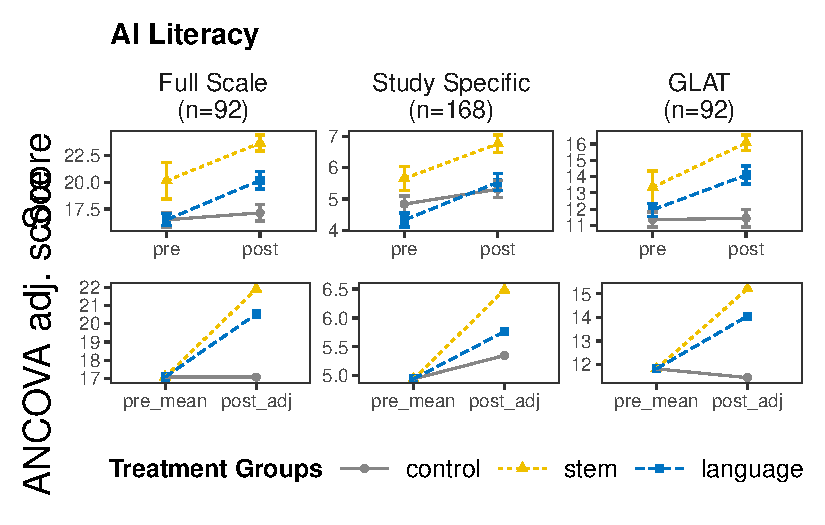
\includegraphics[width=1\textwidth,height=\textheight]{WoLKE-Study_files/figure-latex/fig-ai-lit-1.pdf}

}

\caption{\label{fig-ai-lit}Descriptive Statistics of Students' AI
Literacy Scores Over Time by Treatment Group.}

\end{figure}%

\begin{figure}

\centering{

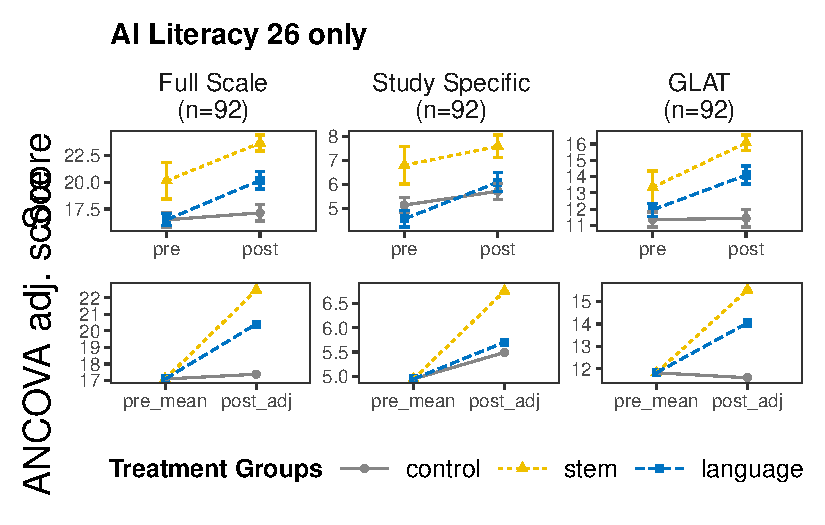
\includegraphics[width=1\textwidth,height=\textheight]{WoLKE-Study_files/figure-latex/fig-ai-lit26-1.pdf}

}

\caption{\label{fig-ai-lit26}Descriptive Statistics of Students' AI
Literacy Scores Over Time by Treatment Group.}

\end{figure}%

\begin{verbatim}
Warning: To compile a LaTeX document with this table, the following commands must be placed in the document preamble:

\usepackage{tabularray}
\usepackage{float}
\usepackage{graphicx}
\usepackage{codehigh}
\usepackage[normalem]{ulem}
\UseTblrLibrary{booktabs}
\UseTblrLibrary{siunitx}
\newcommand{\tinytableTabularrayUnderline}[1]{\underline{#1}}
\newcommand{\tinytableTabularrayStrikeout}[1]{\sout{#1}}
\NewTableCommand{\tinytableDefineColor}[3]{\definecolor{#1}{#2}{#3}}

To disable `siunitx` and prevent `modelsummary` from wrapping numeric entries in `\num{}`, call:

options("modelsummary_format_numeric_latex" = "plain")
 This warning appears once per session.
\end{verbatim}

\begin{table}

\caption{\label{tbl-ancova-ailit-summary}Summary of Multiple Regression
Models for AI Literacy.}

\centering{

\begin{tabular}{lllllllllllll}
& AILIT26 &  &  &  & AILITwolke &  &  &  & AILITglat &  &  &  \\
& β & SE & t & p & β & SE & t & p & β & SE & t & p \\
(Intercept) & \num{-1.57}*** & \num{0.43} & \num{-3.64} & \num{<0.001} & \num{-1.41}*** & \num{0.25} & \num{-5.58} & \num{<0.001} & \num{-1.32}** & \num{0.40} & \num{-3.28} & \num{0.001} \\
intervention-c+STEM\_language & \num{0.74}*** & \num{0.18} & \num{4.11} & \num{<0.001} & \num{0.33}* & \num{0.14} & \num{2.38} & \num{0.018} & \num{0.83}*** & \num{0.19} & \num{4.43} & \num{<0.001} \\
intervention-STEM+language & \num{-0.36} & \num{0.23} & \num{-1.56} & \num{0.122} & \num{-0.45}* & \num{0.19} & \num{-2.34} & \num{0.021} & \num{-0.44}+ & \num{0.24} & \num{-1.81} & \num{0.074} \\
pretest & \num{0.07}* & \num{0.03} & \num{2.63} & \num{0.010} & \num{0.17}*** & \num{0.03} & \num{5.20} & \num{<0.001} & \num{0.10}* & \num{0.04} & \num{2.49} & \num{0.015} \\
gender-f+m & \num{-0.07} & \num{0.19} & \num{-0.36} & \num{0.716} & \num{-0.06} & \num{0.16} & \num{-0.37} & \num{0.714} & \num{-0.18} & \num{0.20} & \num{-0.90} & \num{0.372} \\
semester & \num{0.06} & \num{0.05} & \num{1.10} & \num{0.276} & \num{0.07}* & \num{0.03} & \num{2.50} & \num{0.014} & \num{0.04} & \num{0.05} & \num{0.81} & \num{0.422} \\
Num.Obs. & \num{92} &  &  &  & \num{168} &  &  &  & \num{92} &  &  &  \\
R2 & \num{0.360} &  &  &  & \num{0.272} &  &  &  & \num{0.345} &  &  &  \\
R2 Adj. & \num{0.322} &  &  &  & \num{0.250} &  &  &  & \num{0.307} &  &  &  \\
AIC & \num{233.1} &  &  &  & \num{436.4} &  &  &  & \num{235.1} &  &  &  \\
BIC & \num{250.7} &  &  &  & \num{458.3} &  &  &  & \num{252.8} &  &  &  \\
RMSE & \num{0.80} &  &  &  & \num{0.85} &  &  &  & \num{0.80} &  &  &  \\
\end{tabular}

}

\end{table}%

\subsubsection{Pairwise Contrasts Between
Groups}\label{pairwise-contrasts-between-groups}

\begin{verbatim}
$AILIT26
 intervention_pairwise estimate    SE df t.ratio p.value
 control - stem          -0.924 0.211 86  -4.382 <0.0001
 control - language      -0.563 0.219 86  -2.576  0.0117
 stem - language          0.361 0.231 86   1.563  0.1217

Results are averaged over the levels of: gender 

$AILITwolke
 intervention_pairwise estimate    SE  df t.ratio p.value
 control - stem          -0.558 0.163 162  -3.412  0.0008
 control - language      -0.110 0.176 162  -0.624  0.5332
 stem - language          0.448 0.192 162   2.338  0.0206

Results are averaged over the levels of: gender 

$AILITglat
 intervention_pairwise estimate    SE df t.ratio p.value
 control - stem          -1.053 0.224 86  -4.703 <0.0001
 control - language      -0.613 0.224 86  -2.732  0.0076
 stem - language          0.440 0.243 86   1.809  0.0739

Results are averaged over the levels of: gender 
\end{verbatim}

\begin{verbatim}
$AILIT26
 intervention_pairwise estimate    SE df t.ratio p.value
 control - stem          -0.924 0.211 86  -4.382 <0.0001
 control - language      -0.563 0.219 86  -2.576  0.0117
 stem - language          0.361 0.231 86   1.563  0.1217

Results are averaged over the levels of: gender 

$AILITwolke
 intervention_pairwise estimate    SE  df t.ratio p.value
 control - stem          -0.558 0.163 162  -3.412  0.0008
 control - language      -0.110 0.176 162  -0.624  0.5332
 stem - language          0.448 0.192 162   2.338  0.0206

Results are averaged over the levels of: gender 

$AILITglat
 intervention_pairwise estimate    SE df t.ratio p.value
 control - stem          -1.053 0.224 86  -4.703 <0.0001
 control - language      -0.613 0.224 86  -2.732  0.0076
 stem - language          0.440 0.243 86   1.809  0.0739

Results are averaged over the levels of: gender 
\end{verbatim}

\subsubsection{AI Literacy -- Full Scale}\label{ai-literacy-full-scale}

For the full AI literacy scale, students in the intervention groups
showed significantly greater improvement than students in the control
group, \(\beta\) = 0.74, \emph{SE} = 0.18, \emph{t}(86) = 4.11, \emph{p}
\textless{} .001, indicating a large positive effect in favor of the
intervention groups. The two intervention groups did not differ
significantly from each other, \(\beta\) = -0.36, \emph{SE} = 0.23,
\emph{t}(86) = -1.56, \emph{p} = .122.

\subsubsection{AI Literacy -- Study Specific
Subset}\label{ai-literacy-study-specific-subset}

For the study-specific subset of the AI literacy items, we found a
significant small-to-medium-sized effect of treatment condition on
students' gains in AI literacy, \(\beta\) = 0.33, \emph{SE} = 0.14,
\emph{t}(162) = 2.38, \emph{p} = .018, with students in the intervention
groups showing significantly stronger gains than students in the control
group. In addition, the two intervention groups differed significantly,
\(\beta\) = -0.45, \emph{SE} = 0.19, \emph{t}(162) = -2.34, \emph{p} =
.021, with a medium-sized effect in favor of pre-service STEM teachers
compared to pre-service language teachers.

\subsubsection{AI Literacy -- GLAT
Subset}\label{ai-literacy-glat-subset}

For the GLAT subset of the AI literacy items, we found a significant
large effect of treatment condition on students' gains in AI literacy,
\(\beta\) = 0.83, \emph{SE} = 0.19, \emph{t}(86) = 4.43, \emph{p}
\textless{} .001, indicating stronger gains in the intervention groups
than in the control group. The two intervention groups did not differ
significantly, \(\beta\) = -0.44, \emph{SE} = 0.24, \emph{t}(86) =
-1.81, \emph{p} = .074.

As can be seen in Figure~\ref{fig-ai-lit}, students in both intervention
groups showed descriptively stronger increases in AI literacy than
students in the control group. Pairwise post-hoc contrasts showed that
students in the STEM course had significantly higher adjusted posttest
scores than students in the control group on all three AI literacy
outcomes: the full scale, \(\beta\) = -0.92, \emph{SE} = 0.21,
\emph{t}(86) = -4.38, \emph{p} \textless{} .001, the study-specific
subset, \(\beta\) = -0.56, \emph{SE} = 0.16, \emph{t}(162) = -3.41,
\emph{p} \textless{} .001, and the GLAT subset, \(\beta\) = -1.05,
\emph{SE} = 0.22, \emph{t}(86) = -4.70, \emph{p} \textless{} .001.
Students in the language course also had significantly higher adjusted
posttest scores than students in the control group on the full scale,
\(\beta\) = -0.56, \emph{SE} = 0.22, \emph{t}(86) = -2.58, \emph{p} =
.012, and the GLAT subset, \(\beta\) = -0.61, \emph{SE} = 0.22,
\emph{t}(86) = -2.73, \emph{p} = .008, but not on the study-specific
subset, \(\beta\) = -0.11, \emph{SE} = 0.18, \emph{t}(162) = -0.62,
\emph{p} = .533. Finally, students in the STEM course had significantly
higher adjusted posttest scores than students in the language course on
the study-specific subset, \(\beta\) = 0.45, \emph{SE} = 0.19,
\emph{t}(162) = 2.34, \emph{p} = .021, while the corresponding
difference on the GLAT subset was marginally significant, \(\beta\) =
0.44, \emph{SE} = 0.24, \emph{t}(86) = 1.81, \emph{p} = .074.

\subsection{Intelligent TPACK and AI
Ethics}\label{intelligent-tpack-and-ai-ethics}

The descriptive results of students' ratings of perceived knowledge in
Intelligent TPACK and AI ethics as well as the ANCOVA-adjusted predicted
posttest ratings are shown in Figure~\ref{fig-tpack}, and
Table~\ref{tbl-ancova-tpack-summary} lists the results of the ANCOVA. As
can be seen in Figure~\ref{fig-tpack}, all pre-service teachers reported
their intelligent TPACK knowledge to be around the middle of the scale
at the pretest, while the intervention groups reported, on average,
values \emph{significantly} higher than the middle value of the scale at
the posttest.

For all subscales related to Intelligent TPACK, namely Intelligent TK,
Intelligent TPK, Intelligent TCK, Intelligent TPACK, and AI ethics, we
found a significant effect of treatment condition on students'
self-reported posttest ratings. Students in both intervention groups
reported significantly higher posttest ratings than students in the
control group on the Intelligent TPACK-related subscales, whereas the
two intervention groups did not differ significantly from each other,
see Table~\ref{tbl-ancova-tpack-summary} for an overview.

\begin{figure}

\centering{

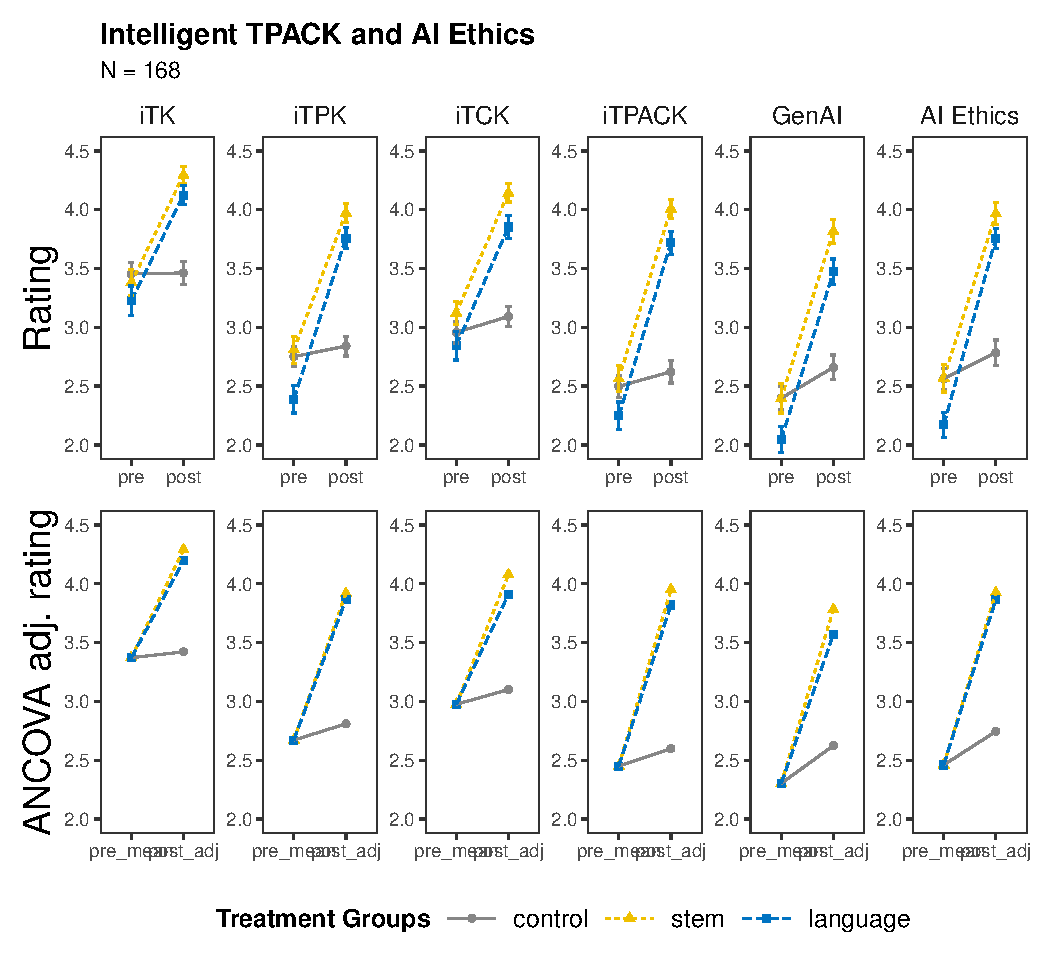
\includegraphics[width=1\textwidth,height=\textheight]{WoLKE-Study_files/figure-latex/fig-tpack-1.pdf}

}

\caption{\label{fig-tpack}Descriptive Statistics of Students'
Intelligent TPACK and AI Ethics Ratings Over Time by Treatment Group.}

\end{figure}%

\begin{figure}

\centering{

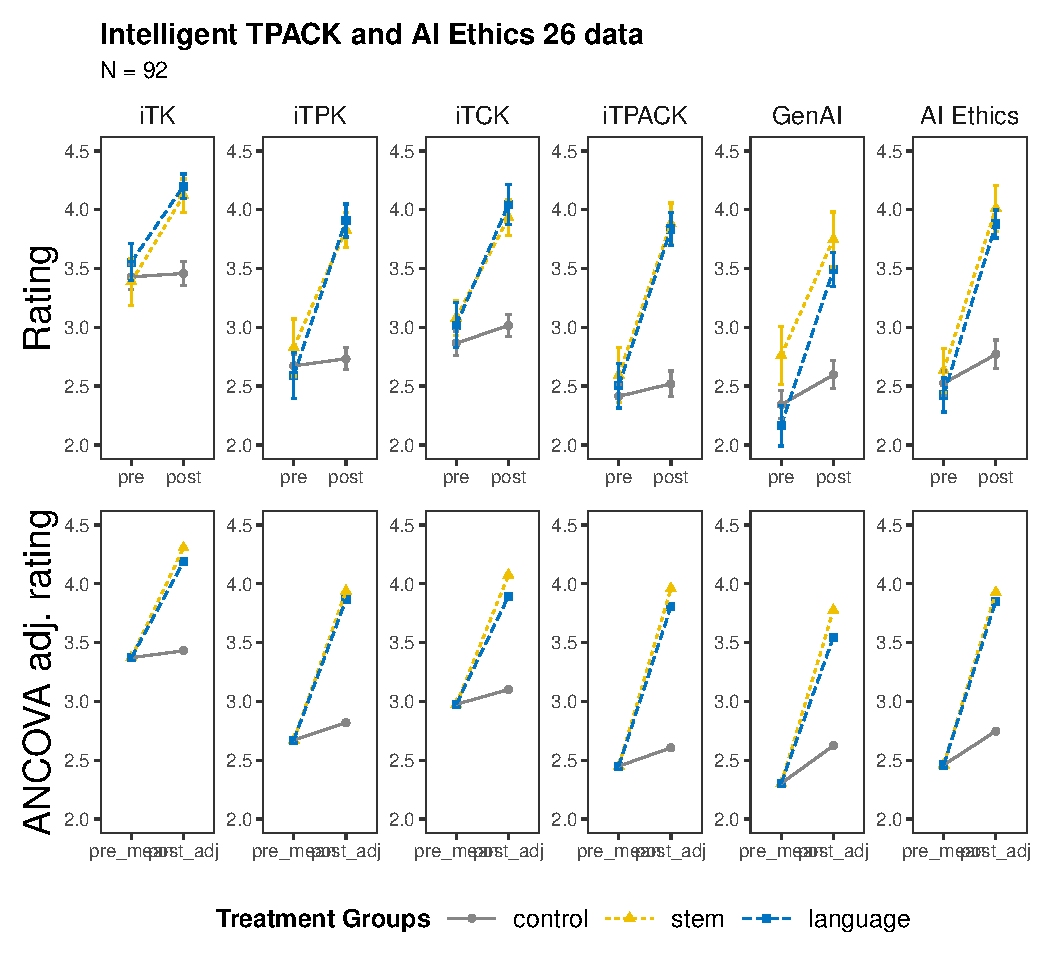
\includegraphics[width=1\textwidth,height=\textheight]{WoLKE-Study_files/figure-latex/fig-tpack26-1.pdf}

}

\caption{\label{fig-tpack26}Descriptive Statistics of Students'
Intelligent TPACK and AI Ethics Ratings Over Time by Treatment Group.}

\end{figure}%

\begin{table}

\caption{\label{tbl-ancova-tpack-summary}Summary of Multiple Regression
Models for Intelligent TPACK Subscales and AI Ethics}

\centering{

\begin{tabular}{lllllllllllllllllllllllll}
& TK &  &  &  & TPK &  &  &  & TCK &  &  &  & TPACKce &  &  &  & TPACKgenai &  &  &  & Ethics &  &  &  \\
& β & SE & t & p & β & SE & t & p & β & SE & t & p & β & SE & t & p & β & SE & t & p & β & SE & t & p \\
(Intercept) & \num{-2.15}*** & \num{0.34} & \num{-6.31} & \num{<0.001} & \num{-1.23}*** & \num{0.32} & \num{-3.89} & \num{<0.001} & \num{-1.47}*** & \num{0.32} & \num{-4.52} & \num{<0.001} & \num{-1.20}*** & \num{0.29} & \num{-4.10} & \num{<0.001} & \num{-0.77}** & \num{0.28} & \num{-2.72} & \num{0.007} & \num{-0.88}** & \num{0.31} & \num{-2.79} & \num{0.006} \\
intervention-c+STEM\_language & \num{1.06}*** & \num{0.12} & \num{9.13} & \num{<0.001} & \num{1.30}*** & \num{0.11} & \num{11.77} & \num{<0.001} & \num{1.09}*** & \num{0.11} & \num{9.88} & \num{<0.001} & \num{1.35}*** & \num{0.10} & \num{13.54} & \num{<0.001} & \num{1.10}*** & \num{0.12} & \num{9.05} & \num{<0.001} & \num{1.23}*** & \num{0.12} & \num{10.23} & \num{<0.001} \\
intervention-STEM+language & \num{-0.11} & \num{0.14} & \num{-0.78} & \num{0.435} & \num{-0.07} & \num{0.16} & \num{-0.45} & \num{0.653} & \num{-0.11} & \num{0.17} & \num{-0.66} & \num{0.507} & \num{-0.10} & \num{0.14} & \num{-0.75} & \num{0.455} & \num{-0.11} & \num{0.18} & \num{-0.63} & \num{0.532} & \num{-0.01} & \num{0.16} & \num{-0.09} & \num{0.928} \\
pretest & \num{0.64}*** & \num{0.07} & \num{8.74} & \num{<0.001} & \num{0.47}*** & \num{0.08} & \num{5.97} & \num{<0.001} & \num{0.54}*** & \num{0.08} & \num{6.94} & \num{<0.001} & \num{0.53}*** & \num{0.07} & \num{7.90} & \num{<0.001} & \num{0.40}*** & \num{0.08} & \num{5.23} & \num{<0.001} & \num{0.41}*** & \num{0.09} & \num{4.69} & \num{<0.001} \\
gender-f+m & \num{0.07} & \num{0.14} & \num{0.52} & \num{0.606} & \num{0.01} & \num{0.13} & \num{0.09} & \num{0.931} & \num{0.23}* & \num{0.11} & \num{2.07} & \num{0.040} & \num{0.11} & \num{0.12} & \num{0.91} & \num{0.364} & \num{0.28}* & \num{0.14} & \num{2.03} & \num{0.043} & \num{0.13} & \num{0.14} & \num{0.90} & \num{0.367} \\
semester & \num{0.01} & \num{0.02} & \num{0.63} & \num{0.532} & \num{0.01} & \num{0.02} & \num{0.60} & \num{0.551} & \num{0.00} & \num{0.02} & \num{0.14} & \num{0.885} & \num{0.01} & \num{0.03} & \num{0.34} & \num{0.737} & \num{0.00} & \num{0.03} & \num{0.10} & \num{0.919} & \num{0.00} & \num{0.03} & \num{0.14} & \num{0.888} \\
Num.Obs. & \num{168} &  &  &  & \num{168} &  &  &  & \num{168} &  &  &  & \num{168} &  &  &  & \num{168} &  &  &  & \num{168} &  &  &  \\
R2 & \num{0.523} &  &  &  & \num{0.522} &  &  &  & \num{0.515} &  &  &  & \num{0.619} &  &  &  & \num{0.428} &  &  &  & \num{0.446} &  &  &  \\
R2 Adj. & \num{0.508} &  &  &  & \num{0.507} &  &  &  & \num{0.500} &  &  &  & \num{0.607} &  &  &  & \num{0.411} &  &  &  & \num{0.429} &  &  &  \\
AIC & \num{365.4} &  &  &  & \num{365.8} &  &  &  & \num{368.4} &  &  &  & \num{327.5} &  &  &  & \num{395.9} &  &  &  & \num{390.5} &  &  &  \\
BIC & \num{387.3} &  &  &  & \num{387.7} &  &  &  & \num{390.2} &  &  &  & \num{349.4} &  &  &  & \num{417.7} &  &  &  & \num{412.4} &  &  &  \\
RMSE & \num{0.69} &  &  &  & \num{0.69} &  &  &  & \num{0.69} &  &  &  & \num{0.62} &  &  &  & \num{0.75} &  &  &  & \num{0.74} &  &  &  \\
\end{tabular}

}

\end{table}%

\subsubsection{Intelligent TK}\label{intelligent-tk}

For Intelligent TK, students in the intervention groups reported
significantly greater improvement than students in the control group,
\(\beta\) = 1.06, \emph{SE} = 0.12, \emph{t}(162) = 9.13, \emph{p}
\textless{} .001, indicating a large positive effect in favor of the
intervention groups. The two intervention groups did not differ
significantly from each other, \(\beta\) = -0.11, \emph{SE} = 0.14,
\emph{t}(162) = -0.78, \emph{p} = .435.

\subsubsection{Intelligent TPK}\label{intelligent-tpk}

For Intelligent TPK, students in the intervention groups reported
significantly greater improvement than students in the control group,
\(\beta\) = 1.30, \emph{SE} = 0.11, \emph{t}(162) = 11.77, \emph{p}
\textless{} .001, indicating a large positive effect in favor of the
intervention groups. The two intervention groups did not differ
significantly from each other, \(\beta\) = -0.07, \emph{SE} = 0.16,
\emph{t}(162) = -0.45, \emph{p} = .653.

\subsubsection{Intelligent TCK}\label{intelligent-tck}

For Intelligent TCK, students in the intervention groups reported
significantly greater improvement than students in the control group,
\(\beta\) = 1.09, \emph{SE} = 0.11, \emph{t}(162) = 9.88, \emph{p}
\textless{} .001, indicating a large positive effect in favor of the
intervention groups. The two intervention groups did not differ
significantly from each other, \(\beta\) = -0.11, \emph{SE} = 0.17,
\emph{t}(162) = -0.66, \emph{p} = .507.

\subsubsection{Intelligent TPACK Core}\label{intelligent-tpack-core}

For the Intelligent TPACK core subscale, students in the intervention
groups reported significantly greater improvement than students in the
control group, \(\beta\) = 1.35, \emph{SE} = 0.10, \emph{t}(162) =
13.54, \emph{p} \textless{} .001, indicating a large positive effect in
favor of the intervention groups. The two intervention groups did not
differ significantly from each other, \(\beta\) = -0.10, \emph{SE} =
0.14, \emph{t}(162) = -0.75, \emph{p} = .455.

\subsubsection{Intelligent TPACK (GenAI)}\label{intelligent-tpack-genai}

For Intelligent TPACK related to GenAI, students in the intervention
groups reported significantly greater improvement than students in the
control group, \(\beta\) = 1.10, \emph{SE} = 0.12, \emph{t}(162) = 9.05,
\emph{p} \textless{} .001, indicating a large positive effect in favor
of the intervention groups. The two intervention groups did not differ
significantly from each other, \(\beta\) = -0.11, \emph{SE} = 0.18,
\emph{t}(162) = -0.63, \emph{p} = .532.

\subsubsection{AI Ethics}\label{ai-ethics}

For AI ethics, students in the intervention groups reported
significantly greater improvement than students in the control group,
\(\beta\) = 1.23, \emph{SE} = 0.12, \emph{t}(162) = 10.23, \emph{p}
\textless{} .001, indicating a large positive effect in favor of the
intervention groups. The two intervention groups did not differ
significantly from each other, \(\beta\) = -0.01, \emph{SE} = 0.16,
\emph{t}(162) = -0.09, \emph{p} = .928.

\subsection{Critical Evaluation of AI
(CEA)}\label{critical-evaluation-of-ai-cea}

todo: 1) daten beschreiben - help me out here 2) ancova ergebnisse
zusammenfassen For the CEA scale and its subscales, we found a
significant effect of treatment condition on students' self-reported
posttest ratings. Students in both intervention groups reported
significantly higher posttest ratings than students in the control group
on the overall CEA scale, CEA understanding, and CEA pedagogical use,
see \textbf{?@tbl-ancova-cea-summary} for an overview.

\begin{tcolorbox}[enhanced jigsaw, breakable, colback=white, opacitybacktitle=0.6, colbacktitle=quarto-callout-note-color!10!white, leftrule=.75mm, colframe=quarto-callout-note-color-frame, toprule=.15mm, opacityback=0, coltitle=black, bottomrule=.15mm, bottomtitle=1mm, toptitle=1mm, titlerule=0mm, title=\textcolor{quarto-callout-note-color}{\faInfo}\hspace{0.5em}{Note}, arc=.35mm, rightrule=.15mm, left=2mm]

Note für uns: ggf. reduzieren wir CEA auf eine Skala mit 9 Items. Im
Piloten haben wir 15 items getestet und EFA hat gezeigt, dass Reduktion
auf 2 Skalen möglich wäre. Das haben wir gemacht, und die funktionieren
auch, aber ein Item lädt z.B. ziemlich stark auf die andere Skala.
Entweder bekommt man das gut begründet, aber den richtigen Mehrwert sehe
ich nicht, 2 Skalen aufzustellen. So oder so, es haben alle Skalen gut
funktioniert und zeigen den Mehrwert vom Seminar. Ggf. einfach auf eine
Full Scale runterbrechen, sagen dass man den fragebogen soweit möglich
evaluiert hat, items reduziert hat und das reicht dann.

\end{tcolorbox}

\begin{verbatim}
Warning: Removed 456 rows containing non-finite outside the scale range
(`stat_summary()`).
Removed 456 rows containing non-finite outside the scale range
(`stat_summary()`).
Removed 456 rows containing non-finite outside the scale range
(`stat_summary()`).
\end{verbatim}

\begin{figure}

\centering{

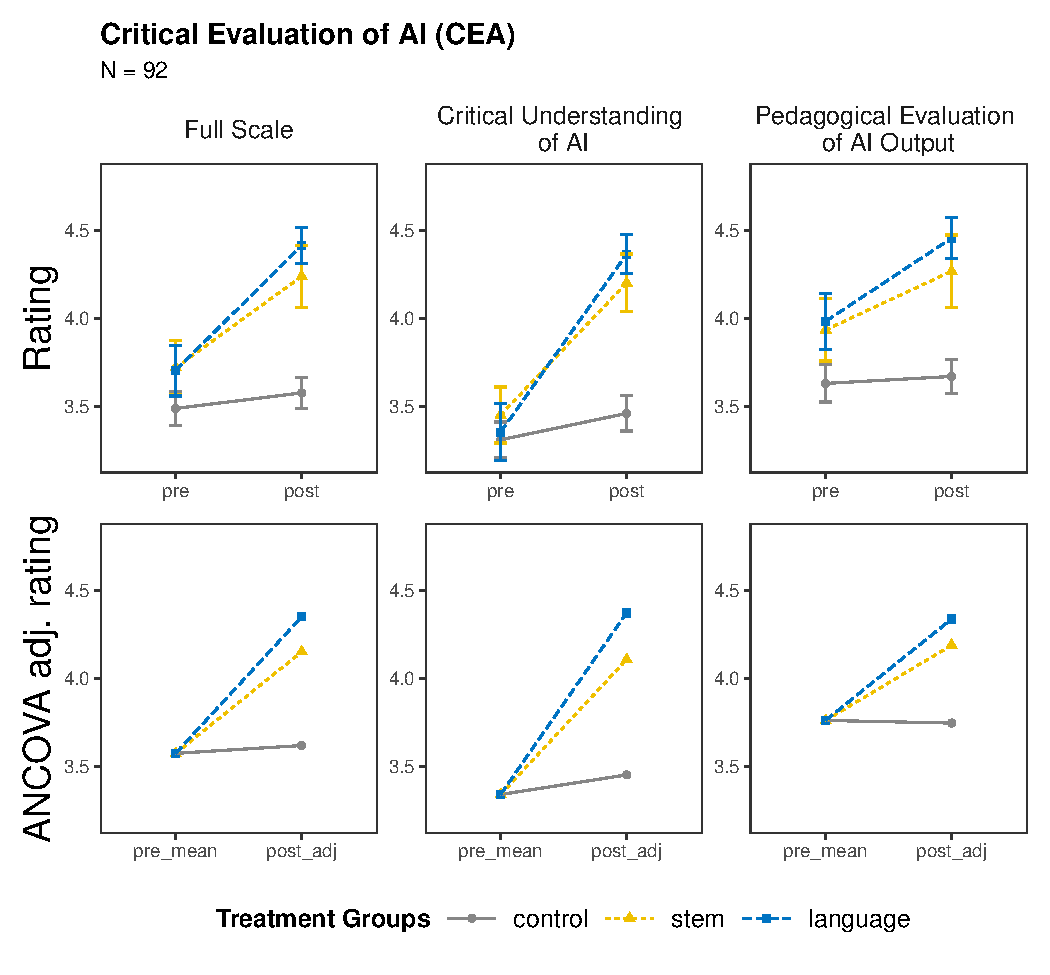
\includegraphics[width=1\textwidth,height=\textheight]{WoLKE-Study_files/figure-latex/fig-cea-1.pdf}

}

\caption{\label{fig-cea}Descriptive Statistics of Students' Critical
Evaluation of AI Over Time by Treatment Group.}

\end{figure}%

\begin{table}

\caption{\label{tbl-ancova-CEA-summary}Summary of Multiple Regression
Models for CEA subscale.}

\centering{

\begin{tabular}{lllllllllllll}
& CEA &  &  &  & CEA\_understanding &  &  &  & CEA\_ped &  &  &  \\
& β & SE & t & p & β & SE & t & p & β & SE & t & p \\
(Intercept) & \num{-2.50}*** & \num{0.56} & \num{-4.46} & \num{<0.001} & \num{-2.03}*** & \num{0.49} & \num{-4.12} & \num{<0.001} & \num{-2.34}*** & \num{0.63} & \num{-3.72} & \num{<0.001} \\
intervention-c+STEM\_language & \num{0.86}*** & \num{0.18} & \num{4.93} & \num{<0.001} & \num{0.99}*** & \num{0.17} & \num{5.74} & \num{<0.001} & \num{0.67}*** & \num{0.19} & \num{3.58} & \num{<0.001} \\
intervention-STEM+language & \num{0.29} & \num{0.29} & \num{0.99} & \num{0.324} & \num{0.31} & \num{0.29} & \num{1.07} & \num{0.287} & \num{0.24} & \num{0.29} & \num{0.83} & \num{0.409} \\
pretest & \num{0.75}*** & \num{0.12} & \num{6.15} & \num{<0.001} & \num{0.61}*** & \num{0.11} & \num{5.53} & \num{<0.001} & \num{0.70}*** & \num{0.13} & \num{5.28} & \num{<0.001} \\
gender-f+m & \num{0.06} & \num{0.22} & \num{0.25} & \num{0.800} & \num{0.04} & \num{0.20} & \num{0.19} & \num{0.850} & \num{0.08} & \num{0.24} & \num{0.32} & \num{0.750} \\
semester & \num{0.01} & \num{0.04} & \num{0.16} & \num{0.871} & \num{0.03} & \num{0.03} & \num{0.85} & \num{0.396} & \num{-0.01} & \num{0.04} & \num{-0.21} & \num{0.835} \\
Num.Obs. & \num{92} &  &  &  & \num{92} &  &  &  & \num{92} &  &  &  \\
R2 & \num{0.540} &  &  &  & \num{0.486} &  &  &  & \num{0.486} &  &  &  \\
R2 Adj. & \num{0.514} &  &  &  & \num{0.456} &  &  &  & \num{0.456} &  &  &  \\
AIC & \num{202.6} &  &  &  & \num{212.8} &  &  &  & \num{212.8} &  &  &  \\
BIC & \num{220.2} &  &  &  & \num{230.4} &  &  &  & \num{230.4} &  &  &  \\
RMSE & \num{0.67} &  &  &  & \num{0.71} &  &  &  & \num{0.71} &  &  &  \\
\end{tabular}

}

\end{table}%

\subsubsection{CEA}\label{cea}

For the overall CEA scale, students in the intervention groups reported
significantly greater improvement than students in the control group,
\(\beta\) = 0.86, \emph{SE} = 0.18, \emph{t}(86) = 4.93, \emph{p}
\textless{} .001, indicating a large positive effect in favor of the
intervention groups. The two intervention groups did not differ
significantly from each other, \(\beta\) = 0.29, \emph{SE} = 0.29,
\emph{t}(86) = 0.99, \emph{p} = .324.

\subsubsection{CEA Understanding}\label{cea-understanding}

For CEA understanding, students in the intervention groups reported
significantly greater improvement than students in the control group,
\(\beta\) = 0.99, \emph{SE} = 0.17, \emph{t}(86) = 5.74, \emph{p}
\textless{} .001, indicating a large positive effect in favor of the
intervention groups. The two intervention groups did not differ
significantly from each other, \(\beta\) = 0.31, \emph{SE} = 0.29,
\emph{t}(86) = 1.07, \emph{p} = .287.

\subsubsection{CEA Pedagogical Use}\label{cea-pedagogical-use}

For CEA pedagogical use, students in the intervention groups reported
significantly greater improvement than students in the control group,
\(\beta\) = 0.67, \emph{SE} = 0.19, \emph{t}(86) = 3.58, \emph{p}
\textless{} .001, indicating a medium-to-large positive effect in favor
of the intervention groups. The two intervention groups did not differ
significantly from each other, \(\beta\) = 0.24, \emph{SE} = 0.29,
\emph{t}(86) = 0.83, \emph{p} = .409.

\subsection{CEA Validity}\label{cea-validity}

The newly developed CEA scale showed good internal consistency at
pretest, Cronbach's α = .86. Internal consistency was acceptable for CEA
understanding, α = .66, and good for CEA pedagogical use, α = .83. The
data were suitable for factor analysis, KMO = .87; Bartlett's test:
χ²(36) = 518.49, \emph{p} \textless{} .001. Parallel analysis suggested
a two-factor solution. The two-factor EFA showed acceptable fit, χ²(19)
= 29.23, \emph{p} = .062, CFI = .982, RMSEA = .079, and explained 63.9\%
of the variance, broadly supporting a two-dimensional structure of the
scale.

\begin{verbatim}
 raw_alpha std.alpha   G6(smc) average_r      S/N        ase     mean        sd
 0.8555533 0.8599656 0.8912677 0.4055916 6.141104 0.01704271 3.576087 0.6904448
 median_r
 0.397035
\end{verbatim}

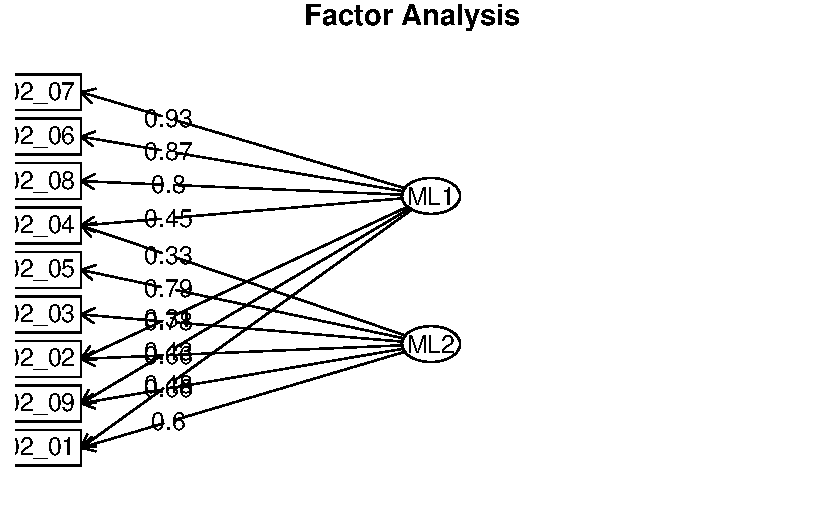
\includegraphics{WoLKE-Study_files/figure-latex/Exploring CEA data-1.pdf}

\begin{verbatim}
This is lavaan 0.6-21 -- running exploratory factor analysis

  Estimator                                         ML
  Rotation method                   VARIMAX ORTHOGONAL
  Rotation algorithm (rstarts)                GPA (30)
  Standardized metric                             TRUE
  Row weights                                   Kaiser

  Number of observations                            92
  Number of missing patterns                         1

Fit measures:
                    aic      bic    sabic  chisq df pvalue   cfi rmsea
  nfactors = 2 1866.465 1954.728 1844.248 29.229 19  0.062 0.982 0.079

Eigenvalues correlation matrix:

    ev1     ev2     ev3     ev4     ev5     ev6     ev7     ev8     ev9 
  4.986   1.394   0.746   0.554   0.381   0.330   0.268   0.217   0.124 

Standardized loadings: (* = significant at 1% level)

            f1      f2       unique.var   communalities
RE02_01  0.604*  0.479*           0.406           0.594
RE02_02  0.656*  0.306*           0.476           0.524
RE02_03  0.783*      .            0.383           0.617
RE02_04  0.328*  0.445*           0.694           0.306
RE02_05  0.787*      .*           0.319           0.681
RE02_06      .*  0.873*           0.193           0.807
RE02_07      .*  0.925*           0.080           0.920
RE02_08      .*  0.797*           0.310           0.690
RE02_09  0.656*  0.425*           0.389           0.611

                              f2    f1 total
Sum of sq (ortho) loadings 3.018 2.732 5.750
Proportion of total        0.525 0.475 1.000
Proportion var             0.335 0.304 0.639
Cumulative var             0.335 0.639 0.639
\end{verbatim}

\subsection{Two Groups (Control
vs.~Intervention)}\label{two-groups-control-vs.-intervention}

\begin{table}

\caption{\label{tbl-ancova-two-groups}Summary of Multiple Linear
Regression Models for Two Treatment Groups.}

\centering{

\begin{tabular}{lllllllllllllllllllllllllllllllllllllllllllllllllllll}
& AILIT26 &  &  &  & AILITwolke &  &  &  & AILITglat &  &  &  & TK &  &  &  & TPK &  &  &  & TCK &  &  &  & TPACKce &  &  &  & TPACKgenai &  &  &  & Ethics &  &  &  & CEA &  &  &  & CEA\_understanding &  &  &  & CEA\_ped &  &  &  & PU &  &  &  \\
& β & SE & t & p & β & SE & t & p & β & SE & t & p & β & SE & t & p & β & SE & t & p & β & SE & t & p & β & SE & t & p & β & SE & t & p & β & SE & t & p & β & SE & t & p & β & SE & t & p & β & SE & t & p & β & SE & t & p \\
(Intercept) & \num{-2.12}*** & \num{0.41} & \num{-5.12} & \num{<0.001} & \num{-1.56}*** & \num{0.25} & \num{-6.31} & \num{<0.001} & \num{-1.91}*** & \num{0.39} & \num{-4.89} & \num{<0.001} & \num{-2.82}*** & \num{0.35} & \num{-8.05} & \num{<0.001} & \num{-2.09}*** & \num{0.33} & \num{-6.31} & \num{<0.001} & \num{-2.17}*** & \num{0.33} & \num{-6.65} & \num{<0.001} & \num{-2.08}*** & \num{0.30} & \num{-6.99} & \num{<0.001} & \num{-1.48}*** & \num{0.30} & \num{-4.93} & \num{<0.001} & \num{-1.69}*** & \num{0.33} & \num{-5.08} & \num{<0.001} & \num{-3.09}*** & \num{0.53} & \num{-5.81} & \num{<0.001} & \num{-2.69}*** & \num{0.47} & \num{-5.74} & \num{<0.001} & \num{-2.80}*** & \num{0.60} & \num{-4.65} & \num{<0.001} & \num{-3.72}*** & \num{0.88} & \num{-4.25} & \num{<0.001} \\
treatmentintervention & \num{0.71}*** & \num{0.18} & \num{3.84} & \num{<0.001} & \num{0.34}* & \num{0.14} & \num{2.42} & \num{0.017} & \num{0.80}*** & \num{0.19} & \num{4.13} & \num{<0.001} & \num{1.06}*** & \num{0.12} & \num{9.17} & \num{<0.001} & \num{1.31}*** & \num{0.11} & \num{11.83} & \num{<0.001} & \num{1.09}*** & \num{0.11} & \num{9.98} & \num{<0.001} & \num{1.35}*** & \num{0.10} & \num{13.57} & \num{<0.001} & \num{1.10}*** & \num{0.12} & \num{9.10} & \num{<0.001} & \num{1.23}*** & \num{0.12} & \num{10.22} & \num{<0.001} & \num{0.88}*** & \num{0.17} & \num{5.32} & \num{<0.001} & \num{1.01}*** & \num{0.17} & \num{6.06} & \num{<0.001} & \num{0.69}*** & \num{0.18} & \num{3.86} & \num{<0.001} & \num{0.26} & \num{0.24} & \num{1.10} & \num{0.274} \\
pretest & \num{0.08}** & \num{0.03} & \num{2.82} & \num{0.006} & \num{0.19}*** & \num{0.03} & \num{5.89} & \num{<0.001} & \num{0.10}* & \num{0.04} & \num{2.60} & \num{0.011} & \num{0.64}*** & \num{0.07} & \num{8.87} & \num{<0.001} & \num{0.47}*** & \num{0.08} & \num{6.12} & \num{<0.001} & \num{0.54}*** & \num{0.08} & \num{7.06} & \num{<0.001} & \num{0.53}*** & \num{0.07} & \num{7.96} & \num{<0.001} & \num{0.40}*** & \num{0.08} & \num{5.32} & \num{<0.001} & \num{0.41}*** & \num{0.09} & \num{4.79} & \num{<0.001} & \num{0.75}*** & \num{0.12} & \num{6.02} & \num{<0.001} & \num{0.61}*** & \num{0.11} & \num{5.38} & \num{<0.001} & \num{0.70}*** & \num{0.13} & \num{5.22} & \num{<0.001} & \num{0.79}*** & \num{0.17} & \num{4.64} & \num{<0.001} \\
gender-f+m & \num{0.01} & \num{0.18} & \num{0.07} & \num{0.941} & \num{0.06} & \num{0.16} & \num{0.39} & \num{0.696} & \num{-0.08} & \num{0.18} & \num{-0.42} & \num{0.675} & \num{0.10} & \num{0.13} & \num{0.81} & \num{0.418} & \num{0.03} & \num{0.12} & \num{0.25} & \num{0.804} & \num{0.26}* & \num{0.11} & \num{2.35} & \num{0.020} & \num{0.14} & \num{0.11} & \num{1.20} & \num{0.233} & \num{0.31}* & \num{0.13} & \num{2.37} & \num{0.019} & \num{0.13} & \num{0.14} & \num{0.98} & \num{0.330} & \num{-0.01} & \num{0.21} & \num{-0.06} & \num{0.949} & \num{-0.04} & \num{0.20} & \num{-0.19} & \num{0.851} & \num{0.02} & \num{0.22} & \num{0.08} & \num{0.936} & \num{0.37}+ & \num{0.18} & \num{1.99} & \num{0.050} \\
semester & \num{0.06} & \num{0.05} & \num{1.13} & \num{0.263} & \num{0.05}* & \num{0.03} & \num{2.06} & \num{0.041} & \num{0.04} & \num{0.05} & \num{0.85} & \num{0.396} & \num{0.01} & \num{0.02} & \num{0.51} & \num{0.613} & \num{0.01} & \num{0.02} & \num{0.53} & \num{0.595} & \num{-0.00} & \num{0.02} & \num{-0.01} & \num{0.992} & \num{0.01} & \num{0.02} & \num{0.23} & \num{0.818} & \num{-0.00} & \num{0.03} & \num{-0.01} & \num{0.993} & \num{0.00} & \num{0.03} & \num{0.13} & \num{0.896} & \num{0.00} & \num{0.04} & \num{0.11} & \num{0.913} & \num{0.03} & \num{0.03} & \num{0.78} & \num{0.436} & \num{-0.01} & \num{0.05} & \num{-0.24} & \num{0.809} & \num{0.05} & \num{0.03} & \num{1.52} & \num{0.133} \\
Num.Obs. & \num{92} &  &  &  & \num{168} &  &  &  & \num{92} &  &  &  & \num{168} &  &  &  & \num{168} &  &  &  & \num{168} &  &  &  & \num{168} &  &  &  & \num{168} &  &  &  & \num{168} &  &  &  & \num{92} &  &  &  & \num{92} &  &  &  & \num{92} &  &  &  & \num{76} &  &  &  \\
R2 & \num{0.349} &  &  &  & \num{0.249} &  &  &  & \num{0.329} &  &  &  & \num{0.521} &  &  &  & \num{0.521} &  &  &  & \num{0.513} &  &  &  & \num{0.618} &  &  &  & \num{0.427} &  &  &  & \num{0.446} &  &  &  & \num{0.533} &  &  &  & \num{0.478} &  &  &  & \num{0.481} &  &  &  & \num{0.425} &  &  &  \\
R2 Adj. & \num{0.319} &  &  &  & \num{0.231} &  &  &  & \num{0.298} &  &  &  & \num{0.510} &  &  &  & \num{0.510} &  &  &  & \num{0.501} &  &  &  & \num{0.609} &  &  &  & \num{0.413} &  &  &  & \num{0.432} &  &  &  & \num{0.512} &  &  &  & \num{0.454} &  &  &  & \num{0.458} &  &  &  & \num{0.392} &  &  &  \\
AIC & \num{232.6} &  &  &  & \num{439.5} &  &  &  & \num{235.4} &  &  &  & \num{363.9} &  &  &  & \num{364.0} &  &  &  & \num{366.9} &  &  &  & \num{326.1} &  &  &  & \num{394.3} &  &  &  & \num{388.5} &  &  &  & \num{202.0} &  &  &  & \num{212.3} &  &  &  & \num{211.7} &  &  &  & \num{184.7} &  &  &  \\
BIC & \num{247.7} &  &  &  & \num{458.3} &  &  &  & \num{250.5} &  &  &  & \num{382.7} &  &  &  & \num{382.8} &  &  &  & \num{385.6} &  &  &  & \num{344.8} &  &  &  & \num{413.0} &  &  &  & \num{407.3} &  &  &  & \num{217.1} &  &  &  & \num{227.4} &  &  &  & \num{226.8} &  &  &  & \num{198.6} &  &  &  \\
RMSE & \num{0.80} &  &  &  & \num{0.86} &  &  &  & \num{0.81} &  &  &  & \num{0.69} &  &  &  & \num{0.69} &  &  &  & \num{0.70} &  &  &  & \num{0.62} &  &  &  & \num{0.75} &  &  &  & \num{0.74} &  &  &  & \num{0.68} &  &  &  & \num{0.72} &  &  &  & \num{0.72} &  &  &  & \num{0.75} &  &  &  \\
\end{tabular}

}

\end{table}%

\phantomsection\label{refs}
\begin{CSLReferences}{1}{0}
\bibitem[\citeproctext]{ref-arel-bundock2022}
Arel-Bundock, V. (2022). {modelsummary}: Data and model summaries in
{R}. \emph{Journal of Statistical Software}, \emph{103}(1), 1--23.
\url{https://doi.org/10.18637/jss.v103.i01}

\bibitem[\citeproctext]{ref-authorsinprep}
Authors. (in prep.). \emph{Development and {Validation} of a {German
Version} of the {Intelligent-TPACK}}.

\bibitem[\citeproctext]{ref-behling.law2025}
Behling, O., \& Law, K. (2025). \emph{Translating {Questionnaires} and
{Other Research Instruments}}. SAGE Publications, Inc.
\url{https://doi.org/10.4135/9781412986373}

\bibitem[\citeproctext]{ref-blair2025}
Blair, G., Cooper, J., Coppock, A., Humphreys, M., \& Sonnet, L. (2025).
\emph{Estimatr: Fast estimators for design-based inference}.
\url{https://declaredesign.org/r/estimatr/}

\bibitem[\citeproctext]{ref-celik2023}
Celik, I. (2023). Towards {Intelligent-TPACK}: {An} empirical study on
teachers' professional knowledge to ethically integrate artificial
intelligence ({AI})-based tools into education. \emph{Computers in Human
Behavior}, \emph{138}, 107468.
\url{https://doi.org/10.1016/j.chb.2022.107468}

\bibitem[\citeproctext]{ref-WWC2022}
Clearinghouse, W. W. (2022). What works clearinghouse procedures and
standards handbook, version 5.0. US department of education, institute
of education sciences. \emph{National Center for Education Evaluation
and Regional Assistance (NCEE)}.
\url{https://ies.ed.gov/ncee/wwc/Handbooks}

\bibitem[\citeproctext]{ref-heinzen2021}
Heinzen, E., Sinnwell, J., Atkinson, E., Gunderson, T., \& Dougherty, G.
(2021). \emph{Arsenal: An arsenal of 'r' functions for large-scale
statistical summaries}. \url{https://github.com/mayoverse/arsenal}

\bibitem[\citeproctext]{ref-huntington2023}
Huntington-Klein, N. (2023). \emph{Vtable: Variable table for variable
documentation}. \url{https://nickch-k.github.io/vtable/}

\bibitem[\citeproctext]{ref-lenth2025}
Lenth, R. V. (2025). \emph{Emmeans: Estimated marginal means, aka
least-squares means}. \url{https://rvlenth.github.io/emmeans/}

\bibitem[\citeproctext]{ref-levenshtein1966}
Levenshtein, V. I. (1966). Binary {Codes} {Capable} of {Correcting}
{Deletions}, {Insertions} and {Reversals}. \emph{Soviet Physics
Doklady}, \emph{10}(8).
\url{https://nymity.ch/sybilhunting/pdf/Levenshtein1966a.pdf}

\bibitem[\citeproctext]{ref-long2022}
Long, J. A. (2022). \emph{Jtools: Analysis and presentation of social
scientific data}. \url{https://cran.r-project.org/package=jtools}

\bibitem[\citeproctext]{ref-long2000}
Long, J. S., \& Ervin, L. H. (2000). Using heteroscedasticity consistent
standard errors in the linear regression model. \emph{The American
Statistician}, \emph{54}(3), 217--224.
\url{https://doi.org/10.1080/00031305.2000.10474549}

\bibitem[\citeproctext]{ref-marsh2009}
Marsh, H. W., Lüdtke, O., Robitzsch, A., Trautwein, U., Asparouhov, T.,
Muthén, B., \& Nagengast, B. (2009). Doubly-{Latent Models} of {School
Contextual Effects}: {Integrating Multilevel} and {Structural Equation
Approaches} to {Control Measurement} and {Sampling Error}.
\emph{Multivariate Behavioral Research}, \emph{44}(6), 764--802.
\url{https://doi.org/10.1080/00273170903333665}

\bibitem[\citeproctext]{ref-R2024}
R Core Team. (2024). \emph{R: A language and environment for statistical
computing}. R Foundation for Statistical Computing.
\url{https://www.R-project.org/}

\bibitem[\citeproctext]{ref-warnes2023}
Warnes, G. R., Bolker, B., Lumley, T., Magnusson, A., Venables, B.,
Ryodan, G., \& Moeller, S. (2023). \emph{Gtools: Various r programming
tools}. \url{https://github.com/r-gregmisc/gtools}

\bibitem[\citeproctext]{ref-wickham2016}
Wickham, H. (2016). \emph{ggplot2: Elegant graphics for data analysis}.
Springer-Verlag New York. \url{https://ggplot2.tidyverse.org}

\bibitem[\citeproctext]{ref-wickham2024}
Wickham, H., Vaughan, D., \& Girlich, M. (2024). \emph{Tidyr: Tidy messy
data}. \url{https://tidyr.tidyverse.org}

\bibitem[\citeproctext]{ref-xiao2024}
Xiao, N. (2024). \emph{Ggsci: Scientific journal and sci-fi themed color
palettes for 'ggplot2'}. \url{https://nanx.me/ggsci/}

\bibitem[\citeproctext]{ref-zhu2024}
Zhu, H. (2024). \emph{kableExtra: Construct complex table with 'kable'
and pipe syntax}. \url{http://haozhu233.github.io/kableExtra/}

\end{CSLReferences}




\end{document}
